\documentclass[russian,utf8,14pt,simple]{eskdtext}

% - Полуторный интервал
\renewcommand{\baselinestretch}{1.50}
% - Отступ красной строки
\setlength{\parindent}{1.25cm}	
% - Шрифт Times New Roman
\renewcommand{\rmdefault}{ftm}

% - Наименование документа
\ESKDtitle{ }
% - Обозначение документа
\ESKDsignature{ФВС КР. Х.ХХХХХХХ 001 ПЗ}
% - Наименование предприятия
\ESKDcolumnIX{ТУСУР, ФВС, КИБЭВС-1208}
% - Проверил
\ESKDchecker{Давыдова Е.М.}	
% - Литера 
\ESKDletter{У}{}{}
% - Разработал
\ESKDauthor{КИБЭВС-1208}			

% - Убирает точку в списке литературы
\makeatletter
\def\@biblabel#1{#1 }

% - ГОСТ списка литературы
\bibliographystyle{gost780s}

\ESKDsectSkip{subsection}{1em}{1em}
\ESKDsectSkip{section}{1em}{1em}

% - Изменение заголовков
\usepackage{titlesec}
\titleformat{\section}{\normalsize}{\thesection}{1.0em}{}
\titleformat{\subsection}{\normalsize}{\thesubsection}{1.0em}{}
\titleformat{\paragraph}{\normalsize}{\theparagraph}{1.0em}{}

% - Для больших таблиц
\usepackage{longtable}

% - Используем графику в документе
\usepackage[dvips]{graphicx}
\graphicspath{{images/}}

% - Для вставки гиперссылок
\usepackage[colorlinks]{hyperref}

% - Счётчики
\usepackage{eskdtotal}

% - Для переопределения списков
\makeatletter
\renewcommand{\theenumi}{\arabic{enumi}}
\renewcommand{\labelenumi}{\theenumi)}

\begin{document}

\newpage
\ESKDthisStyle{empty}

\begin{center}
Министерство образования и науки Российской Федерации\\
ФЕДЕРАЛЬНОЕ ГОСУДАРСТВЕННОЕ БЮДЖЕТНОЕ ОБРАЗОВАТЕЛЬНОЕ\\
УЧРЕЖДЕНИЕ ВЫСШЕГО ПРОФЕССИОНАЛЬНОГО ОБРАЗОВАНИЯ\\
ТОМСКИЙ ГОСУДАРСТВЕННЫЙ\\
УНИВЕРСИТЕТ СИСТЕМ УПРАВЛЕНИЯ И РАДИОЭЛЕКТРОНИКИ\\
(ФГБОУ ВПО ТУСУР)\\
Кафедра комплексной информационной безопасности электронно-вычислительных систем (КИБЭВС)\\
\end{center}

\begin{tabbing}
XXXXXXXXXXXXXXXXXXXXXXXXXXX \=
XXXXXXXXXXXXXXXX\kill
\> УТВЕРЖДАЮ\\
\> заведующий каф.КИБЭВС\\
\> \underline{\ \ \ \ \ \ \ \ \ \ \ \ \ \ \ \ \ \ \ \ } А.А. Шелупанов\\
\> "\underline{\ \ \ \ \ }"\underline{\ \ \ \ \ \ \ \ \ \ \ \ \ \ \ \ \ \ \ \ } 2013г.\\
\end{tabbing}

\begin{center}
КОМПЬЮТЕРНАЯ ЭКСПЕРТИЗА\\
Отчет по групповому проектному обучению\\
Группа КИБЭВС-1208\\
\end{center}

\begin{tabbing}
XXXXXXXXXXXXXXXXXXXXXXXXXXX \=
XXXXXXXXXXXXXXXX\kill
\> Ответственный исполнитель\\
\> Студент гр. 520-1\\
\> \underline{\ \ \ \ \ \ \ \ \ \ \ \ \ \ \ \ \ \ \ \ } Никифоров Д. С.\\
\> "\underline{\ \ \ \ \ }"\underline{\ \ \ \ \ \ \ \ \ \ \ \ \ \ \ \ \ \ \ \ } 2013г.\\
\ \\
\> Научный руководитель\\
\> Аспирант каф.КИБЭВС\\
\> \underline{\ \ \ \ \ \ \ \ \ \ \ \ \ \ \ \ \ \ \ \ } Гуляев А. И.\\
\> "\underline{\ \ \ \ \ }"\underline{\ \ \ \ \ \ \ \ \ \ \ \ \ \ \ \ \ \ \ \ } 2013г.\\
\end{tabbing}
\vfill
\begin{center}
2013
\end{center}

\newpage
\ESKDthisStyle{empty}
\paragraph{\hfill РЕФЕРАТ \hfill}
Курсовая работа содержит \ESKDtotal{page} страниц, \ESKDtotal{table} таблиц, \ESKDtotal{bibitem} источников.

КОМПЬЮТЕРНАЯ ЭКСПЕРТИЗА, ФОРЕНЗИКА, ЛОГИ, QT, ЖУРНАЛЬНЫЕ ФАЙЛЫ, XML, GIT.

Объектом разработки является автоматизированная система для исследования образов жёстких дисков.

Цель работы - создание автоматизированной системы, предназначенной для экспертизы образов жёстких дисков.

Задачей, поставленной на данный семестр, стало написание автоматизированного экспертизного комплекса, имеющего следующие возможности: 

\begin{enumerate}
\item сбор и анализ событий системных журналов операционной системы;
\item сбор и анализ информации из журналов истории браузеров;
\item сбор и анализ истории переписки мессенджеров;
\item сбор и анализ событий журнальных файлов приложений;
\item обнаружение сетевых параметров системы;
\item поиск файлов по имени.
\end{enumerate}

Достигнутые результаты:% созданы части системы, извлекающие из операционной системы, установленной на жёстком диске, логи системы и логи мессенджеров.

Пояснительная записка выполнена в текстовом редакторе Vim.

\newpage
\ESKDthisStyle{empty}
\paragraph{\hfill Список исполнителей \hfill}
Моргуненко А.В. -- документатор.

Никифоров Д.С. -- программист, ответственный исполнитель, ответственный за написание части системы, работающей с логами системы.

Поляков И.Ю. -- программист, ответственный за написание части системы, работающей с логами мессенджеров.

Пономарёв А.К. -- аналитик.

\newpage
\ESKDstyle{formII}
\renewcommand\contentsname{\hfill Содержание \hfill}
\tableofcontents

\newpage
\ESKDstyle{formIIab}
\section{Введение}

Компьютерно-техническая экспертиза является классом инженерно-\\технических экспертиз, проводимых в целях поиска криминалистически значимой информации на носителях, её всестороннего исследование, и, как следствие, получения доказательственной информации и установления фактов, имеющих значение для уголовных, гражданских и административных дел, сопряжённых с использованием компьютерных технологий. Для проведения компьютерных экспертиз необходима высокая квалификация экспертов, так как при изучении представленных носителей информации, попытке к ним доступа и сбора информации возможно внесение в информационную среду изменений или полная утрата важных данных.

Компьютерная экспертиза, в отличие от компьютерно-технической экспертизы, затрагивает только информационную составляющую, в то время как аппаратная часть и её связь с программной средой не рассматривается.

На протяжении предыдущих семестров нами были рассмотрены такие направления компьютерной экспертизы, как исследование файловых систем, сетевых протоколов, организация работы серверных систем, механизм журналирования событий. Также нами были изучены основные задачи, которые ставятся перед сотрудниками правоохранительных органов, которые проводят компьютерную экспертизу, и набор чуществующих утилит, способных помочь эксперту в проведении компьютерной экспертизы. Было выявлено, что существует множество разрозненных программ, предназначенных для просмотра лог-файлов системы и таких приложений, как мессенджеры и браузеры, но для каждого вида лог-файлов необходимо искать отдельную программу. Так как ни одна из них не позволяет эксперту собрать воедино и просмотреть все логи системы, браузеров и мессенджеров, было решено создать для этой цели собственный автоматизированный комплекс, которому на данный момент нет аналогов.

\section{Назначение и область применения}
Разрабатываемый комплекс предназначен для автоматизированного сбора информации из журналов операционных систем и приложений.

\section{Технические характеристики}
\subsection{Постановка задачи}
Для того, чтобы уменьшить время проведения компьютерной экспертизы, необходимо автоматизировать части этого процесса. В данном семестре мы занимались автоматизацией сбора информации из лог-файлов операционной системы Windows. В результате были автоматизированы такие процессы, как сбор информации из журнальных файлов системы и сбор информации из файлов, в которых хранится история переписки мессенджеров skype и pidgin.

\subsection{Выбор единого формата выходных файлов}
XML - eXtensible Markup Language или расширяемый язык разметки. XML разрабатывался как язык с простым формальным синтаксисом, удобный для создания и обработки документов программами и одновременно удобный для чтения и создания документов человеком. Задумка языка в том, что он позволяет дополнять данные метаданными, которые разделяют документ на объекты с атрибутами. Это позволяет упростить программную обработку документов, так как структурирует информацию.

\section{Архитектура}
\subsection{Основной алгоритм}
В ходе разарботки был применен видоизменнённый шаблон проектирования Factory method.

%Описание шаблона и его модификации
Данный шаблон относится к классу порождающих шаблонов. Шаблоны данного класса - это шаблоны проектирования, которые абстрагируют процесс инстанцирования (создания экземпляра класса). Они позволяют сделать систему независимой от способа создания, композиции и представления объектов. Шаблон, порождающий классы, использует наследование, чтобы изменять инстанцируемый класс, а шаблон, порождающий объекты, делегирует инстанцирование другому объекту.
Основной алгоритм представлен на рисунке \ref{architech:architech}.

\begin{figure}[h!]
\center{\includegraphics[width=0.9\linewidth]{architech}}
\caption{Основной алгоритм}
\label{architech:architech}
\end{figure}

Использование данного шаблона позволило нам разбить наш проект на независимые модули, что весьма упростило задачу разработки, так как написание алгоритма для конкретного таска не влияло на остальную часть проекта. При разработке был реализован базовый класс для работы с образом диска. Данный клас предназначался для формирования списка настроек, определения операционной системы на смонтированном образе и инстанционировании и накапливание всех необходимых классов-тасков в очереди тасков. После чего каждый таск из очереди отправлялся на выполнение. Блоксхема работы алгоритма (тут картинка alg_main.eps)

Каждый класс-таск порождался путем наследования от базового абстрактного класса который имеет 8 методов и 3 атрибута:

\begin{enumerate}
\item QString manual() - возвращает справку о входных параметрах данного таска;
\item void setOption(QStringList list) - установка флагов для поданных на вход параметров;
\item QString command() - возвращает команду для инициализации такска вручную;
\item bool supportOS(const coex::typeOS \&os) - возвращает флаг, указывающий на возможность использования данного таска для конкретной операционной системы;
\item QString name() - возвращает имя данного таска;
\item QString description() - возвращает краткое описание таска;
\item bool test() - предназначена для теста на доступность таска;
\item bool execute(const coex::config \&config) - запуск таска на выполнение;
\item QString m\_strName - хранит имя таска;
\item QString m\_strDescription - хранит описание таска;
\item bool m\_bDebug - флаг для параметра --debug;
\end{enumerate}

На данный момент в проекте используется восемь классов. UML-диаграмма классов представлена на рисунке (тут картинка UML.eps)

Классы taskSearchSyslogsWin, taskSearchPidginWin и taskSearchSkypeWin - наследники от класса task являются тасками. Класс winEventLog и _EVENTLOGRECORD предназначины для конвертации журнальных файлов операционной системы Windows XP, а класс writerMessages для преобразования истории переписки.

\newpage
\section{Разработка программного обеспечения}

\subsection{Cбор и анализ истории переписки мессенджеров} % - Отчёт Игоря

\section{TaskSearchArchive}

\subsection{Структура RAR архива}
RAR — проприетарный формат сжатия данных и условно-бесплатная программа-архиватор. Имеет расширение .rar, .rev, .r00 или .r01

Определение архивного файла RAR
RAR-архив состоит из блоков переменной длины с заголовками по 7 байт каждый. Любой архив содержит как минимум два блока MARK_HEAD и MAIN_HEAD. Первый содержит информацию о том, что перед нами RAR, и выглядит как \"0x 52 61 72 21 1A 07 00\" в HEX\'ах, или 0x 52 45 7E 5E” в старых версиях . Третий байт 0х72 как раз таки указывает на то, что это Marker Header. Слово 00 07 в little-endian содержит длину блока. Как раз таки 7 байт.[1]

Второй блок Main Header начинается сразу же после первого и должен содержать 13 байт и иметь маркировочный байт равным 0x73. После него в файле уже начинаются данные — будь-то сжатый файл (маркет 0х74 в третьем байте заголовка блока), комментарий к архиву, дополнительная информация или, к примеру, recovery-запись.[2]

Формат архивного файла RAR
                
Файл архива состоит из блоков разной длины.
В самом начале архива стоит блок-маркер, после которого идёт блок заголовка архива, за которым в произвольном порядке следуют блоки остальных типов.
                
                Каждый блок начинается со следующих полей:         
%Это таблица                 
HEAD_CRC --2 байта --CRC всего блока или его части
HEAD_TYPE --1 байт --Тип блока 
HEAD_FLAGS --16 бит ( =2 байта)--Флаги(*) блока     
HEAD_SIZE --2 байта --Размер блока 
ADD_SIZE --4 байта --Добавление к размеру блока
%конец таблицы 
            
Во всех блоках следующие биты в HEAD_FLAGS (*) имеют одинаковое значение:         
предпоследний 14-й (смещение 0х4000) — если = true (*), то старые версии RAR будут игнорировать этот блок и удалять его при изменении архива; иначе блок копируется в новый архивный файл при изменении архива;
последний 15-й (смещение 0х8000) — если = true, то поле ADD_SIZE присутствует в блоке, иначе — отсутствует.
                
Заявленные типы блоков (возможные значения HEAD_TYPE):             
\begin{itemize}
\item 0x72 (*) — блок-маркер;
\item 0x73 — заголовок архива;
\item 0x74 — заголовок файла;
\item 0x75 — заголовок комментария старого типа;
\item 0x76 — электронная подпись старого типа;
\item 0x77 — субблок старого типа;
\item 0x78 — информация для восстановления старого типа;
\item 0x79 — электронная подпись старого типа;
\item 0x7A — субблок.
\end{itemize}

Форматы блоков
Блок-маркер (MARK_HEAD)
\begin{itemize}
\item HEAD_CRC = 0x6152;
\item HEAD_TYPE = 0x72;
\item HEAD_FLAGS = 0x1a21;
\item HEAD_SIZE = 0x0007;
\end{itemize}

Заголовок архива (MAIN_HEAD)
\begin{itemize}
\item HEAD_CRC = CRC полей от HEAD_TYPE до RESERVED2;
\item HEAD_TYPE = 0x73;
\item HEAD_FLAGS ( =16 бит):                     
\end{itemize}

0-й бит (*) (смещение 0x0001 (*)) — Атрибут тома (том многотомного архива) (*)
1-й бит (смещение 0x0002) — Присутствует архивный комментарий (RAR 3.x использует отдельный блок комментария и не устанавливает этот флаг)
2-й бит (смещение 0x0004) — если = true, то архив заблокирован для изменений
3-й бит (смещение 0x0008) — если = true, то это — непрерывный (solid) архив
4-й бит (смещение 0x0010) — если = true, то используется новая схема именования томов ('volname.partN.rar'), иначе — старая ('volname.rN')
5-й бит (смещение 0x0020) — Присутствует информация об авторе или электронная подпись (AV) (RAR 3.x не устанавливает этот флаг)
6-й бит (смещение 0x0040) — Присутствует информация для восстановления
7-й бит (смещение 0x0080) — Заголовки блоков зашифрованы
8-й бит (смещение 0x0100) — Первый том (устанавливает только RAR 3.0 и выше)
Остальные биты (с 9 по 15-й) зарезервированы для внутреннего использования

\begin{itemize}
\item HEAD_SIZE (*) = Общий размер архивного заголовка, включая архивные комментарии;
\item RESERVED1 (2 байта) - Зарезервировано;
\item RESERVED2 (4 байта) - Тоже зарезервировано;
\end{itemize}

\subsection{Структура ZIP архива}                

ZIP файл состоит из трех областей:
сжатые/несжатые данные, (последовательность структур Local File Header, сами данные и необязательных Data descriptor)
центральный каталог (последовательность структур Central directory file header)
описание центрального каталога (End of central directory record)
С начала файла идет набор из Local File Header, непосредственно данные и (необязательно) структура Data descriptor. Затем структуры типа Central directory file header для каждого файла и папки в ZIP архиве и завершает все это структура End of central directory record.
Local File Header
Используется для описания метаданных файла (имя файла, контрольная сумма, время и дата модификации, сжатый/несжатый размер). Как правило сразу после этой структуры следует содержимое файла.
struct LocalFileHeader
\begin{itemize}
    \item uint32_t signature;	// Обязательная сигнатура, равна 0x04034b50
    \item uint16_t versionToExtract;	// Минимальная версия для распаковки
    \item uint16_t generalPurposeBitFlag;	// Битовый флаг
    \item uint16_t compressionMethod;	// Метод сжатия (0 - без сжатия, 8 - deflate)
    \item uint16_t modificationTime;	// Время модификации файла
    \item uint16_t modificationDate;	// Дата модификации файла
    \item uint32_t crc32;				// Контрольная сумма
    \item uint32_t compressedSize;	// Сжатый размер
    \item uint32_t uncompressedSize;	// Несжатый размер
    \item uint16_t filenameLength;	// Длина название файла
    \item uint16_t extraFieldLength;	// Длина поля с дополнительными данными
    \item uint8_t *filename;			// Название файла (размером filenameLength)
    \item uint8_t *extraField;		// Дополнительные данные (размером extraFieldLength)
\end{itemize}
Сразу после этой структуры идут данные размером compressedSize при использовании сжатия или размером uncompressedSize в противном случае.
Иногда бывает невозможно вычислить данные на момент записи LocalFileHeader, тогда в crc32, compressedSize и uncompressedSize записываются нули третий бит в generalPurposeBitFlag ставится в единицу и после LocalFileHeader добавляется структура типа Data descriptor.
Data descriptor
Если по какой-то причине содержимое файла невозможно создать одновременно с заголовком типа Local File Header, то сразу после него следует структура Data descriptor, где идет находится дополнение метаданных для Local File Header (контрольная сумма, сжатый/несжатый размер). Откровенно говоря, мне такие файлы не попадались, поэтому больше того, чем написано в википедии сказать не могу.
struct DataDescriptor
\begin{itemize}
\item    uint32_t signature;		// Необязательная сигнатура, равна 0x08074b50
\item    uint32_t crc32;			// Контрольная сумма
\item    uint32_t compressedSize;	// Сжатый размер
\item    uint32_t uncompressedSize;	 // Несжатый размер
\end{itemize}
Central directory file header
Расширенное описание метаданных файла. Содержит дополненную версию LocalFileHeader (добавляются поля номер диска, файловые атрибуты, смещение до Local File Header от начала ZIP файла).
struct CentralDirectoryFileHeader
\begin{itemize}
    // Обязательная сигнатура, равна 0x02014b50 
\item    uint32_t signature;    // Версия для создания
\item    uint16_t versionMadeBy;    // Минимальная версия для распаковки
\item    uint16_t versionToExtract;    // Битовый флаг
\item    uint16_t generalPurposeBitFlag;    // Метод сжатия (0 - без сжатия, 8 - deflate)
\item    uint16_t compressionMethod;    // Время модификации файла
\item    uint16_t modificationTime;    // Дата модификации файла
\item    uint16_t modificationDate;    // Контрольная сумма
\item    uint32_t crc32;    // Сжатый размер
\item    uint32_t compressedSize;    // Несжатый размер
\item    uint32_t uncompressedSize;    // Длина название файла
\item    uint16_t filenameLength;    // Длина поля с дополнительными данными
\item    uint16_t extraFieldLength;    // Длина комментариев к файлу
\item    uint16_t fileCommentLength;    // Номер диска
\item    uint16_t diskNumber;    // Внутренние аттрибуты файла
\item    uint16_t internalFileAttributes;    // Внешние аттрибуты файла
\item    uint32_t externalFileAttributes;    // Смещение до структуры LocalFileHeader
\item    uint32_t localFileHeaderOffset;    // Имя файла (длиной filenameLength)
\item    uint8_t *filename;    // Дополнительные данные (длиной extraFieldLength)
\item    uint8_t *extraField;    // Комментарий к файла (длиной fileCommentLength)
\item   uint8_t *fileComment;
\end{itemize}
End of central directory record (EOCD)
Эта структура записывается в конце файла. Содержит следующие поля: номер текущего диска, количество записей Central directory file header в текущем диске, общее количество записей Central directory file header.

\begin{itemize}
// Обязательная сигнатура, равна 0x06054b50
\item uint32_t signature; // Номер диска
\item uint16_t diskNumber;   // Номер диска, где находится начало Central Directory
\item uint16_t startDiskNumber;    // Количество записей в Central Directory в текущем диске
\item uint16_t numberCentralDirectoryRecord;    // Всего записей в Central Directory
\item uint16_t totalCentralDirectoryRecord;    // Размер Central Directory
\item uint32_t sizeOfCentralDirectory;    // Смещение Central Directory
\item uint32_t centralDirectoryOffset;    // Длина комментария
\item uint16_t commentLength;    // Комментарий (длиной commentLength)
\item uint8_t *comment;
\end{itemize}

Папки в ZIP файле представлены двумя структурами Local File Header и Central directory file header с нулевым размером и контрольной суммой. Название папки заканчивается слешем «/».

\subsection{Рефакторинг старого кода :: COEX}
Рефакторинг — это процесс улучшения написанного ранее кода путем такого изменения его внутренней структуры, которое не влияет на внешнее поведение.
Во многом при рефакторинге лучше полагаться на интуицию, основанную на опыте. Тем не менее имеются некоторые видимые проблемы в коде, требующие рефакторинга:
\begin{itemize}
\item дублирование кода;
\item длинный метод;
\item длинный список параметров;
\item «завистливые» функции — это метод, который чрезмерно обращается к данным другого объекта;
\item избыточные временные переменные;
\item классы данных;
\item несгруппированные данные.
\end{itemize}

\subsubsection{Рефакторинг плагина Pidgin}

\begin{itemize}
\item Удаление дублирующегося кода
\item Вынесение блоков кода отвечающих за разбор xml, html логов из TaskPidginWin::execute в отдельные функции (processingLogPidgin, processingContactPidgin, processingAccountPidgin).
\item Замена алгоритма поиска файлов, на более понятный
\item Использование qDebug вместо std::cout
\end{itemize}

\subsubsection{Рефакторинг плагина Skype}

\begin{itemize}
\item Удаление цикличного подключения к БД.
\item Замена алгоритма поиска файлов, на более понятный.
\item Использование qDebug вместо std::cout.
\end{itemize}

\subsection{Совместимость плагинов под формат NoSql БД Solr}

Для совместимости добавления в БД solr необходимо выполнить следующие требования
[https://wiki.apache.org/solr/UpdateXmlMessages]
Документ добавляющий запись в БД имеет следющий формат: 
Корневой тег add,  затем каждая запись/событие помещается в тег doc, где далее/глубже лежат field с нашими  данными. Атрибуты field name определяются разработчиком, в зависимости от необходимости, однако каждая запись должна иметь уникальный id. Так же добавляется в sceme.xml  на сервере solr, для того чтобы БД знала какие данные в нее импортируются, и как с ними работать.
%Таблица
Старый формат
<?xml version=\"1.0\" encoding=\"UTF-8\"?>
<Messages  Messenger=\"pidgin\">
    <info_account name=\"\" email=\"fox.user.3@gmail.com/\" password=\"kpdroscfozyyvsyk\" protocol=\"prpl-jabber\"/>
    <info_account name=\"Игорь Поляков\" email=\"fox.user.3@gmail.com\" password=\"this_is_real_passowrd\" protocol=\"prpl-vkcom\"/>
    <info_account name=\"Игорь Поляков\" email=\"fox.user.3@gmail.com\" password=\"this_is_real_passowrd\" protocol=\"prpl-vkcom\"/>
</Messages >
Новый формат
<?xml version=\"1.0\" encoding=\"UTF-8\"?>
<add>
    <doc>
        <field name=\"id\">pidgin_24d7a3ebd9f601666a7ba27225e71854</field>
        <field name=\"doc_type\">account</field>
        <field name=\"application\">pidgin</field>
        <field name=\"account_id\"></field>
        <field name=\"account_mail\">fox.user.3@gmail.com/</field>
        <field name=\"account_protocol\">prpl-jabber</field>
        <field name=\"account_password\">kpdroscfozyyvsyk</field>
    </doc>
</add>
%Конец таблици
\section{Ссылки}
1 - http://formatsfiles.narod.ru/rar.html
2 - http://www.forensicswiki.org/wiki/RAR

\newpage
\subsection{Отчёт Димы}

\newpage

\chapter*{Введение}

Одной из задач на данный семестр стала задача поиска и переработки журнальных файлов Windows. Сложность данной задачи состоит в том, что все системные события хаписываются в журналы с особой структурой. Существует множество софта, позволяющего просматривать записи из данных журналов, но ни один из рассмотренных проектов не предоставлял открытый исходный код своего приложения. Но обо всем по порядку \\
Для решения данной задачи необходимо было разобратся с такими проблеамами как: \\

\begin{enumerate}
\item определить места хранения журнальных файлов операционной системы
\item изучить какие события записываются в журналы и отбросить ненужные журналы
\item разобраться со структурой журнальных файлов
\item выделить важную информацию их каждой записи журнала
\item автоматизировать процесс поиска журнальных файлов
\item реализовать конвертр журнальных файлов в формат XML
\end{enumerate}

Рассмотрим подробнее каждый этап. \\

\chapter*{Журнльные файлы операционной системы }

Во всех операционных системах Windows начиная с XP есть папка config, в данной папке помимо всего прочего находятся бинарные файлы без расширений из которых формируется реестр системы, а так же файлы с расширением .log и .evt. Как раз эти файлы и являются журналами в которые система записывает некоторые произошедшие события. Какие именно события пишутся зависит от настройки самой системы. \\

В файлы с расширением .log пишется системная информация, размер этих файлов всегда равен 1КБ. А вот файлы с расширением .evt сожержат информацию о подключении/отключении устройств, запуске/остановке программ, ошибок при работе программ, существует так же журнал загрузки операционной системы, журнал обновления системы. Так же опционально можно включить такие журналы как например журналы безопасности и обнаруденных угроз. \\

\charter*{структур .evt файлов}

Файл представляет из себя строки данныйх переменной длинны. Из сторонних источников стало извиестно что некоторые поля данных имеют определенное значение. А именно: \\
Первые 4 байта содержат длинну события в файтах, после длинны идет 4 байтный системный код сообщения. Затем 4байтовы номер записи, после него дата создания записи, время созания, идентификатор события, тип события и так далее. \\

Ниже приведен список полей записи, преднозначенной для счтиывания одного события из журнального файла. \\

	quint32 Length; \\
	quint32 Reserved; \\
	quint32 RecordNumber; \\
	quint32 TimeGenerated; \\
	quint32 TimeWritten; \\
	quint32 EventID; \\
	quint16 EventType; \\
	quint16 NumStrings; \\
	quint16 EventCategory; \\
	quint16 ReservedFlags; \\
	quint32 ClosingRecordNumber; \\
	quint32 StringOffset; \\
	quint32 UserSidLength; \\
	quint32 UserSidOffset; \\
	quint32 DataLength; \\
	quint32 DataOffset; \\

Из сторонних источников стало известно о пяти типах событий (поле EventType): \\

значение - тип события \\

\begin{enumerate}
\item 0x0001 - Error event
\item 0x0010 - Failure Audit event
\item 0x0008 - Success Audit event
\item 0x0004 - Information event
\item 0x0002 - Warning event
\end{enumerate}

У поля EventID удалось определить четыре значения: \\

\begin{enumerate}
\item 0x00 - Success
\item 0x01 - Informational
\item 0x02 - Warning
\item 0x03 - Error
\end{enumerate}

Среди множества полей записи события были выделены поля содержащие информацию о типе события, времени возникновения события и создания записи, пользователя от имени которого была сделана запись, а так же поле Data - поле с бинарными данными в которых записана подробная информация о событии. \\

\charter*{Автоматизация процесса поиска .evt файлов}

Так как комплекс работает с оброзом жесткого диска, то программе достаточно указать папку в которой находятся искомы файлы. Для поиска же можно взять список всех файлов папки и отфилтровать их по расширению .evt. Данную операцию можно сделать при помощи инструметов QDirItherator и QFileInfo из набора библиотек QT. \\

Первый инструмент необходим для получения списка файлов в папке config, а второй позволяет просматривать информацию о файлах. При просмотре иноформации будут отобраны пути до файлов с расширением .evt. После чего список путей будет передан передан процедуре обработки файлов. Которая конвертирует каждый .evt файл в XML и сохранит в диррикторию с результатами работы. Для чтения файла используется инструмент QDataStream, а для записи в XML документ QXmlSreamWriter. \\ 


На данный момент полностью реализован комплекс для работы с журнальными файлами windows XP\\

\charter*{описание используемых инструментов}

Для работы с файловыми системами в QT существует несколько библиотек. В данном проекте активно используются две: \\

\begin{enumerate}
\item QDirIterator
\item QDir
\end{enumerate}

QDirIterator — библотека, предназначенная для работы с файловой системой начиная с определенной директории как точки входа. Создав объект данного типа с указанием директории мы получим все пути которые существуют в файловой системе и начинаются с указанной директории. Данный объект поддерживает фильтрацию которая помогает выделять только необходимую информацию, исключая то, что нас не интересует, например можно вывести список только файлов находящихся в данной директории или поддиректориях, или исключить вывод символьных ссылок. Объекты данного типа используются для поиска файлов или папок на образе исследуемого диска. \\

QDir — библиотека позволяющая работать с конкретной директорией. Создав объект данного типа с указанием директории мы получим доступ к этой директории в программе и сможем работать в ней (просматривать содержимое; удалять, создавать или копировать файлы; создавать поддиректории). Данный объект так же поддерживать разные наборы фильтров выходных данных которые могут отсеивать ненужную информацию. \\

Так же данные библиотеки позволяют создавать объект QFile, который позволяет работать с файлом, путь к которому передается как параметр при создании, данный объект позволяет получить базовую информацию о файле, такую как относительный или абсолютный путь до этого файла, размер файла, тип файла или его имя. Так же позволяет перемещать или копировать данный файл.\\

Работа с xml-файлами \\

XML - eXtensible Markup Language или расширяемый язык разметки. XML разрабатывался как язык с простым формальным синтаксисом, удобный для создания и обработки документов программами и одновременно удобный для чтения и создания документов человеком. Задумка языка в том, что он позволяет дополнять данные метаданными, которые разделяют документ на объекты с атрибутами. Это позволяет упростить программную обработку документов, так как структурирует информацию. \\

В QT для работы с xml-документами используется две библиотеки: \\

\begin{enumerate}
\item QxmlStreamReader
\item QxmlStreamWriter
\end{enumerate}

Данные библиотеки позволяют создавать потоки для чтения и записи XML файлов и предоставляют набор функций для разбиения файлов на элементы и создания структур данных по записям в xml-файлах. \\

Команды для записи же позволяют записывать данные в файл автоматически дополняя методанные. Для этого существует набор команд при помощи которых создается xml-файл с заголовком, команды по созданию элемента, команды по добавлению атрибутов в элемент, команды записи конца элемента и конца файла. \\

<-----
ЗАМЕТКИ
Тут думаю ещё запилить описание написанных классов, зачем нужна каждая функция и добавить выдержки из документации о QDir* QFile* и QXmlStrea*
как источники можно указать:
1) http://doc.crossplatform.ru/qt/ - документация по QT
2) http://www.whitehats.ca/main/members/Malik/malik_eventlogs/malik_eventlogs.html - инфа о структуре evt-файлов
3) Николай Николаевич Федотов - ФОРЕНЗИКА компьютерная криминалистика 2-е издание. - как инфа о экспертизе вообще
с инфой по журналам проблема. я её по кусочкам с каких то левых форумов вытягивал. так что хз что про них можно указать.
----->

\newpage
\section{Отчёт Лёши}

\subsection{Некоторые аспекты сертификации программных средств объектов\\ информатизации по требованиям информационной безопасности}

Под информационной безопасностью объектов информатизации в общем случае понимается такое их состояние, при котором исключается нанесение неприемлемого ущерба субъектам информационных отношений при применении последними средств информатизации. Следовательно, для оценки информационной безопасности объектов информатизации важно оценить сначала степень информационной безопасности средств информатизации, применяемых на объектах информатизации, в том числе всех их компонентов.

Одной из важнейших составляющих любого объекта информатизации являются применяемые программные средства различного назначения, которые существенно влияют на информационную безопасность объекта информатизации в целом.

В настоящее время достаточно полно регламентирована законодательными актами и распорядительными документами организация работ по сертификации средств защиты информации. Разработаны и представлены в виде нормативных документов (Государственных стандартов и Руководящих документов Гостехкомиссии России) требования к защиты информации автоматизированных систем и их компонентов (вычислительных и программных средств). Отработаны методы их проверки и создано достаточно большое количество программных средств для проведения испытаний. Однако в основной их части требования касаются средств и методов защиты информации от несанкционированного доступа, а также проверок на отсутствие закладных деструктивных элементов в таких программных средствах.

В то же время информационная безопасность средств информатизации определяется не только их защищенностью от несанкционированного доступа. Одной из важнейших составляющих является выполнение средством информатизации заданных функций в различных условиях функционирования, в том числе при воздействии внешних деструктивных факторов.

Действительно, стержневой характеристикой качества любого средства информатизации является его функциональная пригодность. Ибо, если средство информатизации не решает в заданном объеме и с заданным качеством установленных для него задач, то нет смысла обеспечивать защиту от несанкционированного доступа и нецелесообразно его применять по назначению, так как только по этой причине результаты его использования могут привести к непредсказуемым последствиям и нанести пользователю неприемлемый ущерб.

В рамках Системы сертификации «Росинфосерт» разрабатывается подход к сертификации средств информатизации по требованиям информационной безопасности, сущность которого основана на действующей нормативно-методической базе Системы сертификации «Росинфосерт». Эта нормативно-методическая база дорабатывается с учетом требований Федерального закона «О техническом регулировании», в том числе в части вычислительных и программных средств, а также компьютерных систем в целом.

В ФЗ «О техническом регулировании» определены типы технических регламентов, в которых должны быть сформулированы требования по обеспечению биологической, механической, пожарной, промышленной, химической и др. видов безопасности применительно к продукции, работам и услугам. К сожалению, не попали в этот список требования по обеспечению информационной безопасности. Очевидно, Законодатель считает ее составной частью всех остальных видов безопасности.

Согласно закону, безопасность продукции определяется ее характеристиками, безопасность работ и предоставляемых услуг определяется применением безопасной продукции и безопасностью методов использования этой продукции при работах и предоставлении услуг. Фактически безопасность продукции является одной из составляющих ее качества.

Таким образом, информационная безопасность средств информатизации должна оцениваться в рамках общей оценки их качества, как один из показателей качества продукции.

При рассмотрении вопросов информационной безопасности исследуется и оценивается безопасность информационных ресурсов (данных, программ и их совокупности), которые, в свою очередь нельзя рассматривать в отрыве от вычислительных средств, на которых они размещены и реализованы. То есть предметом рассмотрения должны быть вычислительные средства с реализуемыми на них информационными ресурсами.

Таким образом, требования информационной безопасности следует применять к многоуровневому программно-вычислительному комплексу как единому целому (рисунок \ref{mnogour_pvk:pon1}):

В характеристики качества (в том числе и в информационную безопасность) такого комплекса компоненты каждого уровня вносят свою составляющую. Например, недостаточная надежность технических компонентов вычислительных средств может компенсироваться программно-алгоритмическими решениями. В конечном счете, следует рассматривать в качестве основного показателя качества комплекса безопасность его функционирования.

Поскольку 100\% безопасности функционирования любого комплекса определенной структуры быть не может, то можно говорить о безопасности комплекса лишь в вероятностном смысле. Это в полной мере относится к компонентам любого уровня.

В общем случае для прикладных программных средств безопасное функционирование означает:

\begin{itemize}
\item полное и точное выполнение всех заданных функций;
\item обеспечение целостности и сохранности;
\item обеспечение защиты от неправильных действий пользователя, от некорректных входных данных, от случайных сбоев вычислительных средств;
\item простой и удобный интерфейс.
\end{itemize}

Эти составляющие обеспечивают как аппаратные средства, так и операционная среда, Однако, центральным моментом оценки качества прикладных программных средств должна являться оценка их собственных функциональных характеристик, но, прежде, чем провести оценку качества прикладных программных средств, следует убедиться в том, что характеристики остальных составляющих комплекса соответствуют предъявляемым к ним требованиям, в том числе требованиям информационной безопасности.

\begin{figure}[h!]
\center{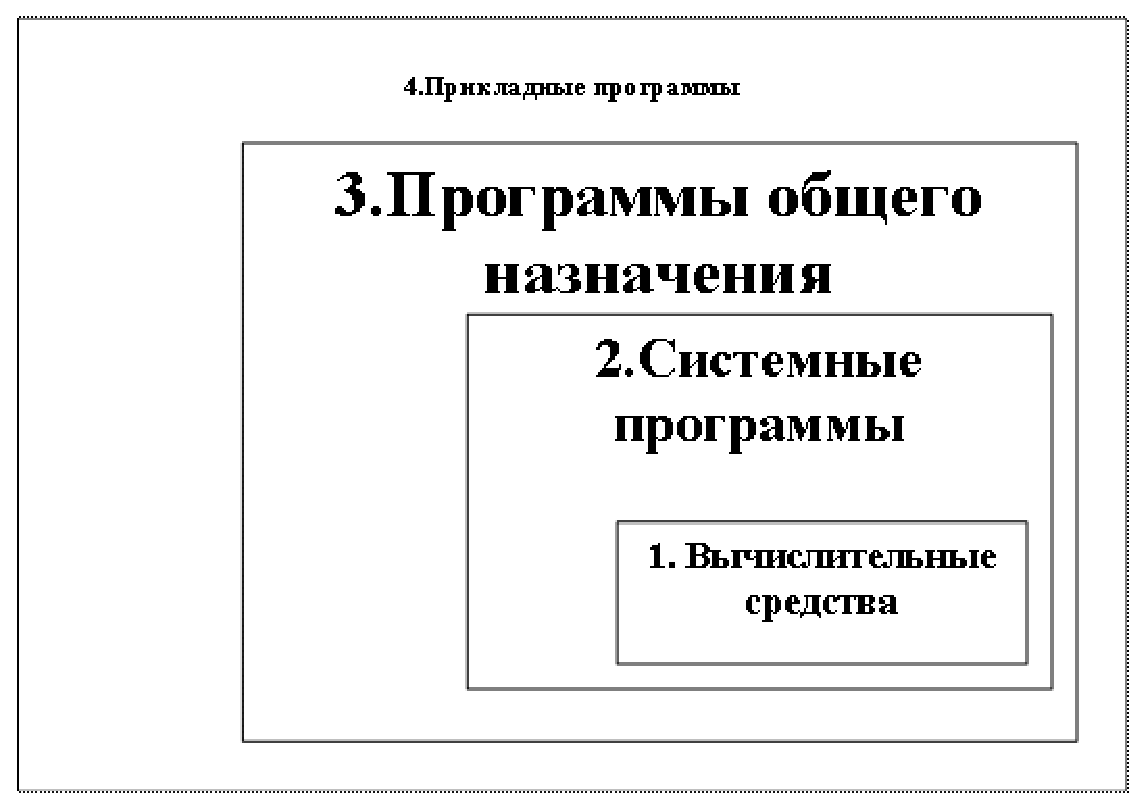
\includegraphics[width=0.6\linewidth]{pon1}}
\caption{Многоуровневый программно-вычислительный комплекс}
\label{mnogour_pvk:pon1}
\end{figure}

В свете всего сказанного предлагается следующая этапность оценки:

1-й этап – осуществляется оценка выполнения требований к качеству комплекса на первом уровне. Здесь исследуются и оцениваются характеристики преимущественно технических средств с использованием широкой номенклатуры специальных или специализированных тестов.

2-й этап – осуществляется оценка уже программно – аппаратного комплекса, включающего средства 1-го и 2-го уровней (технические средства и системные программные средства). При исследованиях и оценках используются имитаторы (в том числе программные) сигналов внешних устройств и функционирования программ общего назначения.

3-й этап – осуществляется оценка программно – аппаратного комплекса, включающего средства 1-го, 2-го и 3-го уровней (технические средства, системные программные средства и программные средства общего назначения). При оценках также используются независимые имитаторы сигналов внешних устройств, функционирования программ общего назначения и прикладных программ.

И, наконец, на 4-м этапе осуществляется оценка характеристик качества всего программно-вычислительного комплекса в целом. При этом используются результаты всех предыдущих этапов, что повышает достоверность и доверие к полученным оценкам.

Обязательные требования к продукции (работам и услугам) по действующему законодательству Российской Федерации устанавливаются Техническими регламентами, принимаемыми в качестве Федеральных законов. Сегодня необходимость технического регламента, устанавливающего обязательные требования по информационной безопасности к программно-вычислительным комплексам очевидна. При этом основным инструментом контроля соблюдения таких требований является сертификация (подтверждение соответствия). Место Системы сертификации в рамках проведения единой технической политики России в области решения задач информатизации поясняется рисунком \ref{sistsert:pon2}.

\begin{figure}[h!]
\center{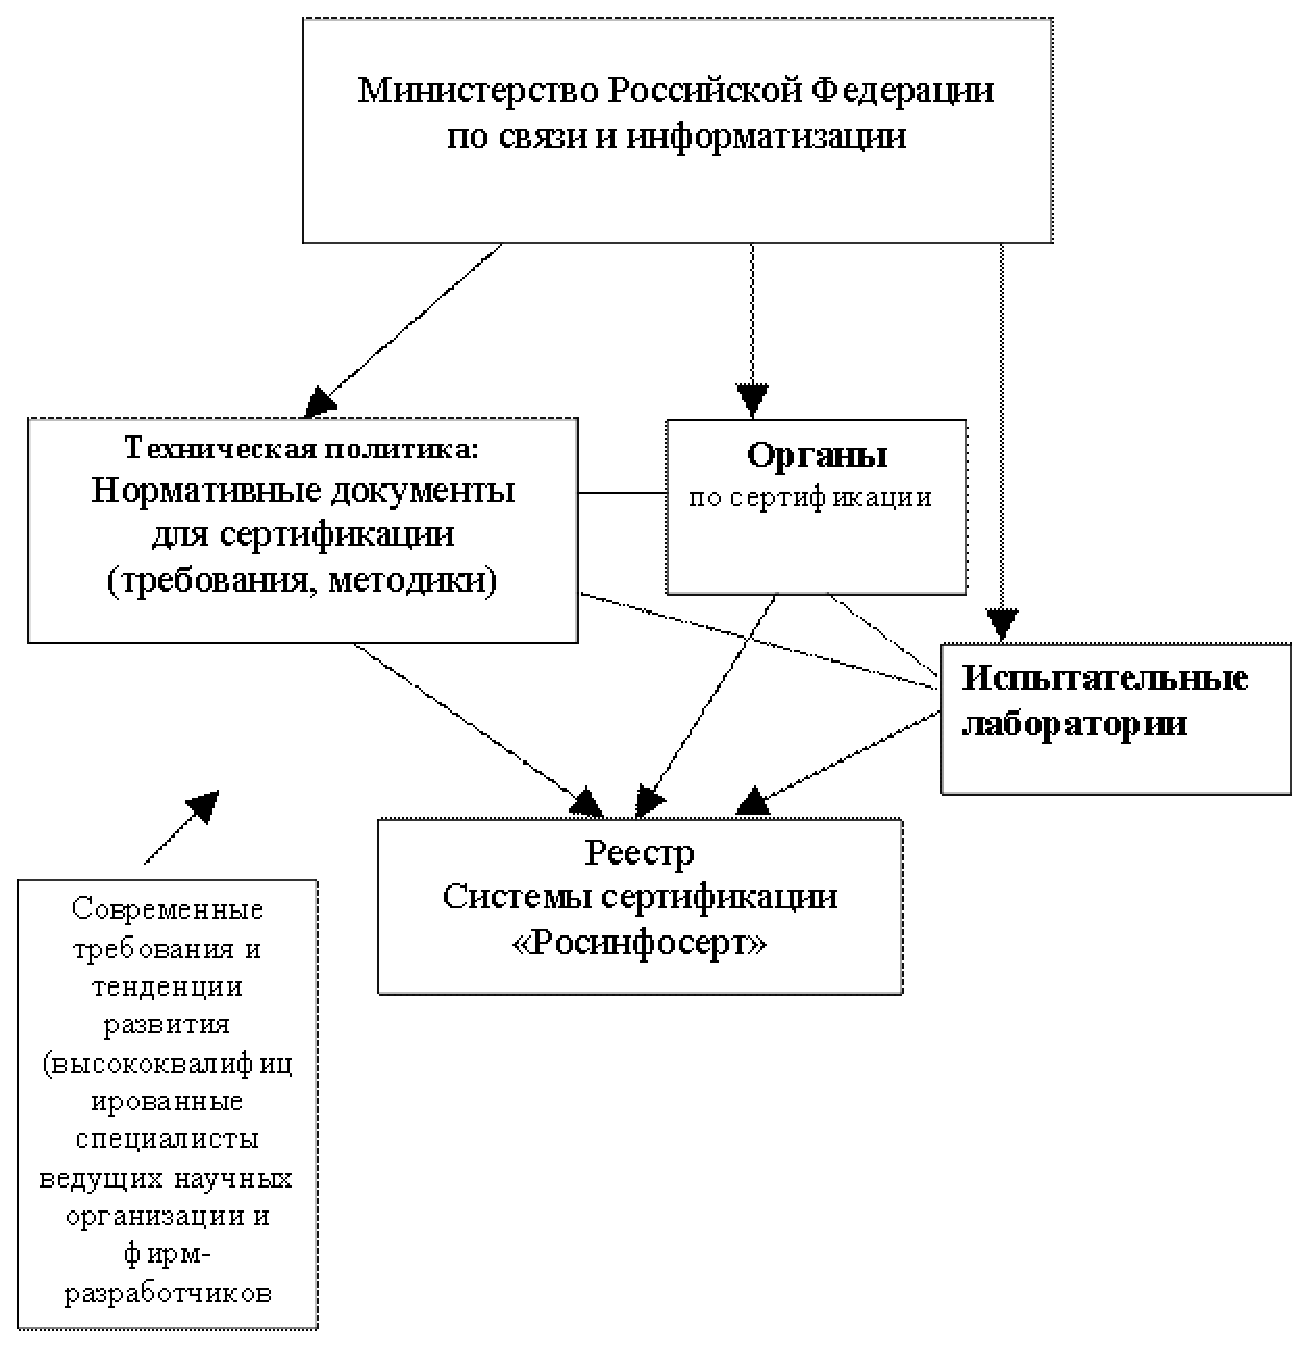
\includegraphics[width=0.8\linewidth]{pon2}}
\caption{Cистема сертификации при проведении единой технической политики}
\label{sistsert:pon2}
\end{figure}

Регистрация в реестре Системы сертифицированной продукции и выдача сертификата соответствия заявителю.
Применение результатов сертификации продукции можно проиллюстрировать примером проведения тендера на поставку средств информатизации для государственных нужд. Схема проведения такого тендера представлена на рисунке \ref{tender:pon3}.

\begin{figure}[h!]
\center{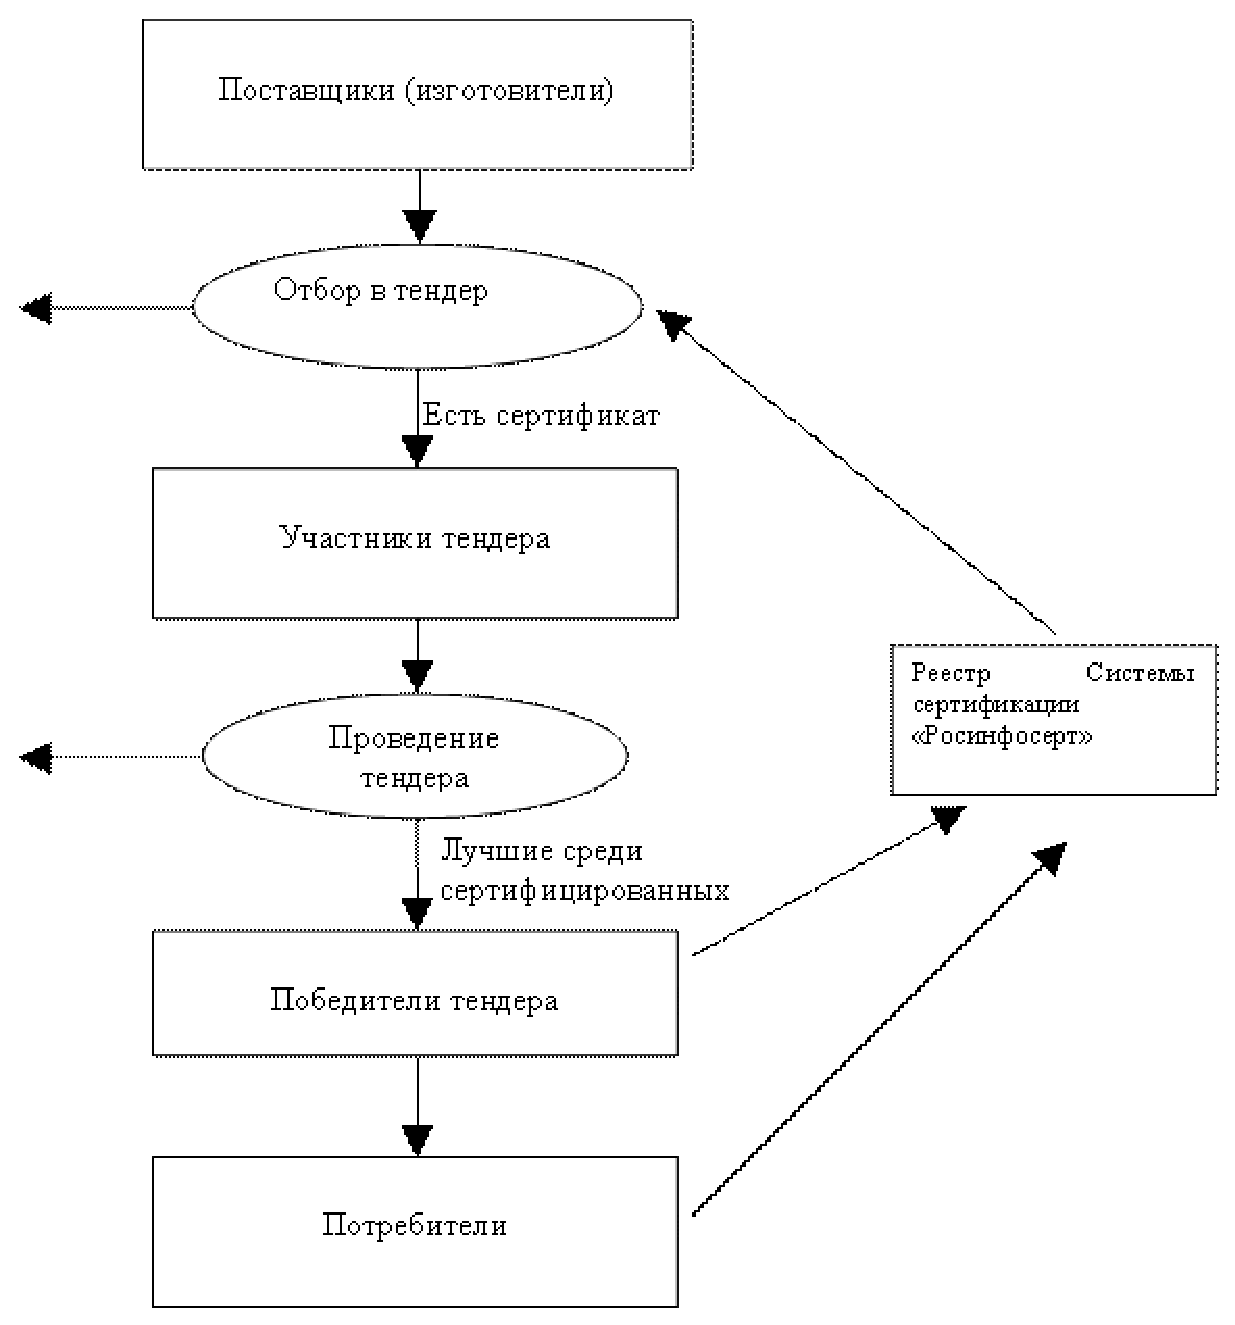
\includegraphics[width=0.8\linewidth]{pon3}}
\caption{Схема проведения тендера на поставку средств информатизации для государственных нужд}
\label{tender:pon3}
\end{figure}

Отбор участников тендера целесообразно проводить на основе анализа результатов их деятельности, одним из объективных показателей которой является сертификат соответствия системы менеджмента качества организации требованиям международных стандартов ИСО 9001 – 2001, а также наличие в номенклатуре выпускаемой продукции сертифицированных продуктов, характеристики которых представлены в Реестре Системы. Такой подход ставит барьер недобросовестным поставщикам и некачественной продукции на рынок средств информатизации России.

В этом случае нормативно-правовое обеспечение применения сертификации для реализации обязательных требований информационной безопасности составляют следующие документы:

\begin{enumerate}
\item Соглашение о взаимодействии в области сертификации средств информатизации между Минсвязи России и субъектом равного уровня. Такое соглашение является необязательным, но желательным документом, который регламентирует взаимоотношения руководства Системы сертификации, ее органов и испытательных лабораторий с потенциальными поставщиками и потребителями средств информатизации, впрямую не подчиняющимися Минсвязи России.
\item Распоряжение (постановление, приказ) субъекта об утверждении Положения о порядке использования средств информатизации для решения своих задач.
\item Положение о порядке использования субъектом средств информатизации, устанавливающее систему показателей и правил отбора и применения поставляемых для государственных нужд средств информатизации.
\item Нормативный документ для сертификации, содержащий состав характеристик средства информатизации, их допустимые значения и способы оценки. Этот документ носит статус стандарта организации, утверждается Минсвязи России по согласованию с субъектом.
\end{enumerate}


\newpage
\section{Заключение}
В результате проделанной работы были достигнуты следующие результаты:

типа ссылка \cite{qtdoc}
типа вторая ссылка \cite{fedotovforenzika}

В дальнейшей работе планируется:
\begin{itemize}
\item добавление части системы, работающей с логами браузеров.
\end{itemize}

\newpage
\renewcommand{\refname}{Список использованных источников}
\bibliography{biblio/lit}

\ESKDappendix{Обязательное}{\normalfont Компакт-диск}
Компакт-диск содержит: 
\begin{itemize}
\item электронную версию пояснительной записки в форматах *.tex и *.pdf;
\item индивидуальные ежемесячные отчеты студентов;
\item групповые ежемесячные отчёты.
\end{itemize}

\end{document}
